\documentclass[11pt,a4paper,fleqn,abstracton]{scrartcl}
\usepackage[T1]{fontenc}
\usepackage{enumerate,sqrt,chimuk,graphicx}
\usepackage[german]{babel}
\usepackage[hang,bf]{caption}

\bibliographystyle{ups}

\def\version{1.0}

\title{Das Upstream-Spline Advektionsverfahren}
\author{Michael Schr"oter}
\date{Version \version{}, \today}


\begin{document}
%
  \maketitle
%
  \nocite{mahrer:78,price:73}
%
\begin{abstract}
     Dokumentation des Upstream-Spline Advektionsverfahrens. Es behandelt die 
     allgemeine Berechnung des Splines und die Berechnung im speziellen bei
     Verwendung bestimmter Randbedingungen. Zus"atzlich wird die L"osung 
     tridiagonaler linearer Gleichungssysteme vorgestellt. Abschlie"send
     wird ein selektiver Filter vorgestellt, der es erm"oglicht sogenannte
     $2\Delta$-Instabilit"aten, welche zum Beispiel bei der Upstream-Spline
     Advektion k"unstlich angeregt werden, auszufiltern. 
\end{abstract}
%
Gesucht ist die L"osung der Advektionsterme in prognostischen Gleichungen, welche hier
f"ur eine allgemeine Gr"o"se $\psi$ und die Raumrichtung $x$ formuliert:
\begin{equation}\label{advek:eq}
\frac{\6\psi}{\6 t}=-u\frac{\6\psi}{\6 x}\;
\end{equation}
lauten.
Ist die advehierende Geschwindigkeit $u$ konstant, so entspricht die L"osung von
(\ref{advek:eq}) der Verlagerung von $\psi$ um die Distanz $u\cdot \Delta t$ 
innerhalb des Zeitintervalls $\Delta t$. Die numerische L"osung von
(\ref{advek:eq}) setzt eine konstante Verlagerungsgeschwindigkeit  w"ahrend eines 
Zeitschritts $\Delta t$ voraus. Entspricht die Verlagerungsdistanz
$u\cdot \Delta t$ nicht dem ganzzahligen Vielfachen der numerischen Gitterweite,
so ist die Anwendung eines Interpolationsverfahrens notwendig, um Werte von $\psi$ 
zwischen den Maschenpunkten zu erhalten.

Der Unterschied zu anderen Advektionsverfahren, wie zum Beispiel dem
\textit{Upstream}-Verfahren oder dem Verfahren von \textit{Piacsek und Williams},
bei denen zur Beschreibung der Advektion eine Approximation von
Differenzenquotienten vorgenommen wird, liegt darin, da"s bei dem
\textit{Upstream-Spline Advektionsverfahren} die Str"omung durch eine
interpolierende Funktion angen"ahert wird. Als interpolierende Funktion setzt das 
\textit{Upstream-Spline Advektionsverfahren} eine
kubische Splinefunktion $s_{\Delta}$ an. Es handelt sich dabei um eine Funktion, 
die auf jedem Teilintervall $[x_{i},x_{i+1}]$, mit $i=0,\ldots,N-1$, zweimal stetig
differenzierbar sind und dort mit einem Polynom dritten Grades "ubereinstimmen.
Eine Splinefunktion ist somit st"uckweise aus $N$ kubischen Polynomen so zusammengesetzt,
da"s die Funktion $s_{\Delta}$ selbst und ihre beiden ersten Ableitungen an den
Stellen $x_i$, mit $i=1,\ldots,N-1$, keine Sprungstellen besitzen 
\comshortcite{stoer:72}. D.~h. an den Randpunkten der Teilintervalle werden die
Splinefunktionen $s_{\Delta,i}$ durch folgende  Beziehungen miteinander verkn"upft:
\begin{eqnarray}
s_{\Delta,i}(x_i)  & = & s_{\Delta,i+1}(x_i) \nonumber \\
s'_{\Delta,i}(x_{i}) & = & s'_{\Delta,i+1}(x_{i}) 
                              \hspace{0.5cm}\mbox{f"ur}\hspace{0.25cm} i=0,\ldots,N\!-\!1\nonumber \\
s''_{\Delta,i}(x_{i}) & = & s''_{\Delta,i+1}(x_{i})\;. \nonumber
\end{eqnarray}
$s_{\Delta,i}(x_i)$ ist hier die auf dem $i$-ten Teilintervall g"ultige 
Splinefunktion und $x_i$ sind die Knotenpunkte (St"utzstellen) des Splines.
Sie entsprechen des Knotenpunkten des numerischen Gitters in die jeweilige
betrachtete Raumrichtung.

Unter Verwendung der Steigungen der Splinefunktionen $m_i$, kann die Splinefunktion
als
\begin{eqnarray}\label{spline_eq}
s_\Delta(x) & = & m_{i-1}\frac{\left(x_i-x\right)^2 \left(x-x_{i-1}\right) }{h_i^2}
                  -m_i\frac{\left(x-x_i\right)^2\left(x_i-x\right)}{h_i^2}\nonumber\\
            &   & +\psi_{i-1}
                      \frac{\left(x_i-x\right)^2\left[2\left( x-x_i\right) +h_i\right]}{h_i^3}
                  +\psi_i
                      \frac{\left(x-x_{i-1}\right)^2\left[2\left(x_i-x\right)+h_i\right]}{h_i^3}
\end{eqnarray}
formuliert werden \comshortcite{ahlberg:67}, mit $h_i=x_i-x_{i-1}=dx_i$. 
F"ur die advehierte Gr"o"se an einem Gitterpunkt $i$ zum Zeitpunkt $t+\Delta t$ gilt
dann:
\begin{equation}
  \psi_i^{t+\Delta t} = s^{t}_\Delta(x+\alpha_i\Delta x)\;,
\end{equation}
mit $\alpha_i=u_i\frac{\Delta t}{\Delta x}$. F"ur $u_i\ge 0$ erh"alt man durch
Einsetzen von $x-\alpha_i$ in (\ref{spline_eq}):
\begin{eqnarray}
  \psi_i^{t+\Delta t} & = &
     \psi_i^{t} - m_i\alpha + \left[
       3\left(\psi_{i-1}^{t}-\psi_i^{t} \right) + 2m_i + m_{i-1}\right]\alpha^2 \\
                      &   & - \left[ m_i + m_{i-1} + 
           2\left( \psi_{i-1}^{t}-\psi_i^{t}\right)\right]\alpha^3\;.
\end{eqnarray}
F"ur $u_i<0$ folgt mit $x+\alpha_i$ (der Spline wird hier zwischen den Punkten $x_i$
und $x_i+1$ ausgewertet):
\begin{eqnarray}
  \psi_i^{t+\Delta t} & = &
     \psi_i^{t} + m_i\alpha + \left[
       3\left(\psi_{i}^{t}-\psi_{i+1}^{t} \right) + 2m_i + m_{i+1}\right]\alpha^2 \\
                      &   & - \left[ m_i + m_{i+1} + 
           2\left( \psi_{i}^{t}-\psi_{i+1}^{t}\right)\right]\alpha^3\;.
\end{eqnarray}

Unter der Voraussetzung, da"s die Splinefunktionen an ihren R"andern stetig
ineinander "ubergehen, ergibt sich folgende Bestimmungsgleichung f"ur die Steigungen
$m_i$:
\begin{equation}
\frac{1}{h_i}m_{i-1}+2\left(\frac{1}{h_i}+\frac{1}{h_{i+1}}\right)m_i+\frac{1}{h_{i+1}}m_{i+1}=
 3\frac{\psi_i-\psi_{i-1}}{h_i^2}+3\frac{\psi_{i+1}-\psi_i}{h_{i+1}^2}\;.
\end{equation}
F"ur $i$ gilt hier $i=1,\ldots,N-1$. Mit
\begin{eqnarray}
\lambda_i & = & \frac{h_{i+1}}{h_i+h_{i+1}}\label{lambda:eq}, \\[8pt]
\mu_i     & = & 1-\lambda_i \label{mu:eq}, \\[8pt]
c_i       & = & 3\frac{\psi_i-\psi_{i-1}}{h_i^2}+3\frac{\psi_{i+1}-\psi_i}{h_{i+1}^2}
\end{eqnarray}
folgt
\begin{equation}\label{spl:eq}
\lambda_i m_{i-1} + 2 m_i + \mu_i m_{i+1} = c_i\;.
\end{equation}

Die R"ander des Modellgebietes m"ussen eine gesonderte Untersuchung
erfahren. Hierzu ist die Formulierung von Randbedingungen notwendig, wobei zwischen
lateralen und vertikalen Randbedingungen unterschieden werden mu"s. Lateral werden in
der LES meist zyklische Randbedingungen angesetzt. Der Index $i$ l"auft hier nicht von 0 bis $N$,
sondern es gilt $i=-1,\ldots ,nx+1$ (f"ur $x$-Richtung). Es gilt:
\[
\psi_{-1} = \psi_{nx}\hspace{1cm}\mbox{und}\hspace{1cm}\psi_{0} = \psi_{nx+1}\;.
\]
In vertikaler Richtung mu"s hingegen zwischen Neumannschen und Dirichletschen 
Randbedingungen unterschieden werden. Der Laufindex f"ur die vertikale 
Richtung bewegt sich in den Grenzen $0\le i\le nz$ und es gilt:
\begin{enumerate}
\item Neumann-R"ander:
\[
\frac{\6 \psi_{0,nz}}{\6 x_i} = 0
\]
\item Dirichlet-R"ander:
\[
\psi_{0,nz}=\psi_0=const
\]
\end{enumerate} 
Jede Wahl der Randbedingung wirkt sich anders auf die Bestimmung der
Splinekoeffizienten $m_i$ aus, wie im folgenden erl"autert wird.

\subsection*{Nichtperiodische Randbedingungen, Advektion in vertikaler Richtung}
F"ur nichtperiodische Splinefunktionen (Neumann oder Dirichlet Randbedingungen) ist
die Angabe zweier zus"atzlicher Randbedingungen f"ur $c$ und $i=0$ bzw.
$i=nz$ notwendig:
\begin{eqnarray}
2 m_{0}+\mu_{0} m_1 = c_{0} & \mbox{f"ur} & i = 0 \nonumber\\
\lambda_{nz} m_{nz-1} + 2 m_{nz} = c_{nz} & \mbox{f"ur} & i = nz
\end{eqnarray}
mit
\[
\mu_{0}= \lambda_{nz}=1
\]
und
\begin{equation}
c_{0}=3\frac{\psi_1-\psi_{0}}{h_1}\hspace{1cm}\mbox{bzw.}\hspace{1cm}
c_{nz}=3\frac{\psi_{nz}-\psi_{nz-1}}{h_{nz}}\;.
\end{equation}
Dies gilt jedoch nur unter der Voraussetzung, da"s die Kr"ummungen der
Ausgangsfunktion $\psi''(x)$ bzw. der Splinefunktionen $s''_\Delta(x)$ an den
R"andern verschwinden. F"ur $i=1,\ldots,nz-1$ gilt weiterhin:
\begin{equation}
c_i=3\lambda_i\frac{\psi_i-\psi_{i-1}}{h_i}+3\mu_i\frac{\psi_{i+1}-\psi_i}{h_{i+1}}\;.
\end{equation}
Die einzige Unbekannte sind hier die Steigungen der Splinefunktionen $m_i$. Zu ihrer
Bestimmung ist die L"osung des folgenden linearen Gleichungssystems notwendig:
\begin{equation}
\begin{array}{ccccccc}
2 m_{0}               & + & \mu_{0} m_{1} &   &              & = & c_{0} \\
\lambda_1 m_{0}       & + & 2 m_1         & + & \mu_1 m_{0}  & = & c_1  \\
                      &   & \vdots        &   &              & = & \vdots \\
\lambda_{nz} m_{nz-1} & + & 2 m_{nz}      &   &              & = & c_{nz}
\end{array}
\end{equation}
bzw.
\begin{equation}
\left(\begin{array}{ccccc}
2            & \mu_{0}  &                &              &  \\
\lambda_1    & 2        & \mu_1          &              &           \\
             & \ddots   & \ddots         & \ddots       &           \\
             &          & \lambda_{nz-1} & 2            & \mu_{nz-1}  \\
             &          &                & \lambda_{nz} & 2    
\end{array}\right)
\cdot
\left(\begin{array}{c}
m_{0} \\ m_1 \\ \vdots \\ m_{nz-1} \\ m_{nz}
\end{array}\right)
=
\left(\begin{array}{c}
c_{0} \\ c_1 \\ \vdots \\ c_{nz-1} \\ c_{nz}
\end{array}\right)
\end{equation}
(leere Pl"atze stehen f"ur Nullen). 
Bei diesem linearen Gleichungssystem ist die Koeffizientenmatrix eine Tridiagonalmatrix mit
konstanten Koeffizienten, die ausschlie"slich von der Struktur des verwendeten 
Modellgitters abh"angen (siehe (\ref{lambda:eq}) und (\ref{mu:eq})).


\subsection*{Periodische Randbedingungen, Advektion in lateraler Richtung}

F"ur zyklische laterale Randbedingungen (periodischer Splineansatz) kann
(\ref{spl:eq}) f"ur $i=0$ und $i=nx$ vollst"andig formuliert werden:
\begin{equation}\label{spl-lgs:eq}
  \begin{array}{ccccccc}
    \lambda_0 m_{-1} & + & 2 m_0  & + & \mu_0 m_{1} & = & c_0 \\
    \lambda_1 m_{0}  & + & 2 m_1  & + & \mu_1 m_{2} & = & c_2  \\
                     &   & \vdots &   &             & = & \vdots \\
    \lambda_{nx} m_{nx-1} & + & 2 m_{nx} & + & \mu_{nx} m_{nx+1} & = & c_{nx}
  \end{array}
\end{equation}
Unter Verwendung der Bedingungen f"ur den zyklischen Rand
\newlength{\savearracs}
\setlength{\savearracs}{\arraycolsep}
\setlength{\arraycolsep}{8pt}
\[
\begin{array}{cccc}
s_\Delta(x_{-1}) = s_\Delta(x_{nx})\,, & 
m_{-1} = m_{nx}\,, & 
s_\Delta(x_{nx+1}) = s_\Delta(x_{0})\,, & 
m_{nx+1} = m_{0}
\end{array}
\]
\setlength{\arraycolsep}{\savearracs}
kann (\ref{spl-lgs:eq}) zu
\begin{equation}
\begin{array}{ccccccc}
\lambda_0 m_{nx} & + & 2 m_0  & + & \mu_0 m_{1} & = & c_0 \\
\lambda_1 m_{0}  & + & 2 m_1  & + & \mu_1 m_{2} & = & c_2  \\
                 &   & \vdots &   &             & = & \vdots \\
\lambda_{nx} m_{nx-1} & + & 2 m_{nx} & + & \mu_{nx} m_{0} & = & c_{nx}
\end{array}
\end{equation}
umgeschrieben werden, was dem L"osen von
\begin{equation}
\left(\begin{array}{ccccc}
2            & \mu_0  &              &              & \lambda_0 \\
\lambda_1    & 2      & \mu_1        &              &           \\
             & \ddots & \ddots       & \ddots       &           \\
             &        & \lambda_{nx-1} & 2            & \mu_{nx-1}  \\
\mu_{nx}     &        &              & \lambda_{nx} & 2    
\end{array}\right)
\cdot
\left(\begin{array}{c}
m_0 \\ m_1 \\ \vdots \\ m_{nx-1} \\ m_{nx}
\end{array}\right)
=
\left(\begin{array}{c}
c_0 \\ c_1 \\ \vdots \\ c_{nx-1} \\ c_{nx}
\end{array}\right)
\end{equation}
"aquivalent ist. Wie auch f"ur den nichtperiodischen Fall sind hier die Koeffizienten
der Matrix nur von der Struktur des numerischen Gitters abh"angig, jedoch ist
die Koeffizientenmatrix keine Tridiagonalmatrix mehr, wodurch sich der Aufwand f"ur
die L"osung des Gleichungssystems erh"oht.

\subsection*{L"osen der linearen Gleichungssysteme}

Sowohl im periodischen als auch im nichtperiodischen Fall kann die Koeffizientenmatrix
vor jeder Simulation einmal zur Verf"ugung gestellt werden und f"ur den Rest
der Simulation unver"andert bleiben. In \textsf{PALM-1} geschieht die 
Bereitstellung der Koeffizientenmatrix nach der "Uberpr"ufung der
Eingabeparameter (\texttt{check\_parameters.f90}) in dem Unterprogramm
\texttt{init\_advec.f90}


\minisec{Die Koeffizientenmatrix im nichtperiodischen Fall}

F"ur tridiagonale Gleichungssysteme verringert sich der Rechenaufwand f"ur das
Standard-Gau"s-L"osungsverfahren (Thomasalgorithmus). Ausgangspunkt f"ur diesen Algorithmus
ist das folgende lineare Gleichungssystem:
\begin{equation}\label{lgs:eq}
\mathsf{A}_{(nz+1)\times (nz+1)}\cdot \vc{m} = \vc{c}\;.
\end{equation}
Dem Standard-Gau"s-L"osungsverfahren folgend wird zun"achst die Matrix
$\mathsf{A}_{(nz+1)\times (nz+1)}$ in eine linke untere Dreiecksmatrix
$\mathsf{L}_{(nz+1)\times (nz+1)}$
und eine rechte obere Dreiecksmatrix $\mathsf{R}_{(nz+1)\times (nz+1)}$ zerlegt.
Da $\mathsf{A}_{(nz+1)\times (nz+1)}$ eine Tridiagonalmatrix ist und alle Elemente
au"ser den Diagonal-, Subdiagonal- und Superdiagonalelementen gleich 0 sind, sind
bei den Matrizen $\mathsf{L}$ und $\mathsf{R}$
auch nur die Diagonal- und Subdiagonal bzw. die Diagonal- und Superdiagonalelemente 
von 0 verschieden. Die Matrizen $\mathsf{L}$ und $\mathsf{R}$ nehmen deshalb folgende
einfache Gestalt an:
\[
\mathsf{L}_{(nz+1)\times (nz+1)} =\left(\begin{array}{lllll}
1             & 0          &        &           &       \\
l_{1}         & 1          & \ddots &           &  \\
              & l_{2}      & 1      & \ddots    &  \\
              &            & \ddots & \ddots    & 0 \\
              &            &        & l_{nz}    & 1
\end{array}\right)
\]
und
\[
\mathsf{R}_{(nz+1)\times (nz+1)} =\left(\begin{array}{lllll}
d_{0}  & r_{0}     &         &             & \\
0      & d_{1}     & r_{1}   &             &  \\
       & \ddots    & d_{2}   & \ddots      &  \\
       &           & \ddots  & \ddots      & r_{nz-1} \\
       &           &         & 0           & d_{nz}
\end{array}\right)\;.
\]
Die Zerlegung der Matrix kann, wie bereits angesprochen, einmalig vor
Beginn der eigentlichen Simulationen vorgenommen werden (\texttt{init\_advec.f90}),
wobei sich die Koeffizienten wie folgt berechnen:
\begin{eqnarray}
d_{0}       & = & a_{0,0}       \\[6pt]
r_{i}       & = & a_{i,i+1}\hspace{1cm}\mbox{mit}\hspace{10pt}i=0,\ldots,nz-1 \\[6pt]
l_{i}       & = & \frac{c_{i}}{d_{i-1}}
                           \hspace{1cm}\mbox{mit}\hspace{10pt}i=1,\ldots,nz \\[6pt]
d_{i}       & = & a_{i,i}-a_{i-1,i}\cdot l_{i}
                           \hspace{1cm}\mbox{mit}\hspace{10pt}i=1,\ldots,nz
\end{eqnarray}
Gel"ost wird das Gleichungssystem (\ref{lgs:eq}) nun in zwei Schritten, denn es gilt:
\[
\mathsf{A}_{(nz+1)\times (nz+1)}\cdot\vc{m} =
\mathsf{L}_{(nz+1)\times (nz+1)}\underbrace{\mathsf{R}_{(nz+1)\times (nz+1)}
 \cdot\vc{m}}_{\dis\glr \vc{y}} = \vc{c}
\]
\begin{enumerate}[\textbf{Schritt} 1:]
\item 
\[
\mathsf{L}_{(nz+1)\times (nz+1)}\cdot\vc{y}=\vc{c}
\]
\item
\[
\mathsf{R}_{(nz+1)\times (nz+1)}\cdot\vc{m}=\vc{y}\;.
\]
\end{enumerate}

\minisec{Die Koeffizientenmatrix im periodischen Fall}

Im periodischen Fall handelt es sich bei der Matrix $\mathsf{A}_{(nx+1)\times (nx+1)}$
um eine sogenannte zyklische Tridiagonalmatrix der Form:
\begin{equation}
\mathsf{A}_{(nx+1)\times (nx+1)}=\left(\begin{array}{ccccccc}
a_{0,0}   & a_{0,1} & 0       & 0      & \cdots      & \beta \\
a_{1,0}   & a_{1,1} & a_{1,2} & 0      & \cdots      & 0           \\
0         & \ddots  & \ddots  & \ddots &             & \vdots      \\
\vdots    & \ddots  & \ddots  & \ddots & \ddots      & 0      \\
0         &         & \ddots  & \ddots & a_{nx-1,nx-1} & a_{nx-1,nx}    \\
\alpha    & 0       & \cdots  & 0      & a_{nx,nx-1}   & a_{nx,nx}
\end{array}\right)\;,
\end{equation}
mit $\alpha=\mu_{nx}$ und $\beta=\lambda_0$.

Gleichungssysteme dieser Form k"onnen mit Hilfe der \textsc{Sherman-Morrison} Formel
\comshortcite{press:86} gel"ost werden, dabei gilt es zwei lineare Gleichungssysteme
zu l"osen:
\begin{eqnarray}
\mathsf{A}_{(nx+1)\times (nx+1)} \cdot \vc{y} & = & \vc{b}\label{lgs-cyc1:eq}\;, \\
\mathsf{A}_{(nx+1)\times (nx+1)} \cdot \vc{z} & = & \vc{u}\label{lgs-cyc2:eq}\;.
\end{eqnarray}
Die endg"ultige L"osung $\vc{m}$ ergibt sich anschlie"send zu:
\begin{equation}
\vc{m}=\vc{y}-\left( \frac{\vc{v}\cdot\vc{y}}{1+(\vc{v}\cdot\vc{z})}\right)\vc{z}\;.
\end{equation}
Die Vektoren $\vc{u}$ und $\vc{v}$ sind dabei wie folgt definiert:
\[
\vc{u} = \left(\begin{array}{c}
          \gamma  \\
           0      \\
           \vdots \\
           0      \\
           \alpha\end{array}\right)\;,\hspace{1cm}
\vc{v} = \left(\begin{array}{c}
           1  \\
           0      \\
           \vdots \\
           0      \\
           \beta/\alpha\end{array}\right)\;.
\]
Der Parameter $\gamma$ kann dabei beliebig gew"ahlt werden. Er wird hier gem"a"s des
Vorschlages von \shortciteN{press:86} zu $\gamma=-a_{0,0}$ gew"ahlt. Wird nun die
Matrix $\mathsf{A}_{(nx+1)\times (nx+1)}$ derart modifiziert, da"s gilt:
\[
a'_{0,0}=a_{0,0}-\gamma\hspace{1cm}\mbox{und}\hspace{1cm}
a'_{nx,nx}=a_{nx,nx}-\frac{\alpha\beta}{\gamma}
\]
und
\[
\mathsf{A}_{(nx+1)\times (nx+1)}=\left(\begin{array}{ccccccc}
a'_{0,0}  & a_{0,1} &         &        &             &  \\
a_{1,0}   & a_{1,1} & a_{1,2} &        &             &  \\
          & \ddots  & \ddots  & \ddots &             &  \\
          &         & \ddots  & \ddots & \ddots      &  \\
          &         &         & \ddots & a_{nx-1,nx-1} & a_{nx-1,nx}    \\
          &         &         &        & a_{nx,nx-1}   & a'_{nx,nx}
\end{array}\right)\;,
\]
so k"onnen die Gleichungen (\ref{lgs-cyc1:eq}) und (\ref{lgs-cyc2:eq}) wie
herk"ommliche tridiagonale Gleichungssysteme behandelt werden.

\minisec{Der Thomasalgorithmus}

Gel"ost werden die linearen Gleichungssysteme sowohl im nichtperiodischen als auch im periodischen
Fall mit dem sogenannten Thomasalgorithmus.
\begin{description}
\item[1. Vorw"artssubstitution:]
\begin{eqnarray}
y_{0}   & = & c_{0}  \hspace{0.5cm}\mbox{\small nichtperiodisch}       \\[6pt]
y_{0}   & = & c_{0}  \hspace{0.5cm}\mbox{\small periodisch}       \\[6pt]
y_{i}   & = & c_{i} - l_{i,i-1}\cdot y_{i-1}
                                \hspace{0.5cm}\mbox{mit}\,
\left\{\begin{array}{lr}
i=1,\ldots,nz & \mbox{\small nichtperiod.} \\
i=0,\ldots,nx & \mbox{\small period.}
\end{array}\right.
\end{eqnarray}
\item[2. R"uckw"artssubstitution:]
\begin{eqnarray}
m_{nz}   & = & \frac{y_{nz}}{d_{nz}}\hspace{0.5cm}\mbox{\small nichtperiodisch}  \\[6pt]
m_{nx}   & = & \frac{y_{nx}}{d_{nx}}\hspace{0.5cm}\mbox{\small periodisch}  \\[6pt]
m_{i}      & = & \frac{y_{i} - r_{i+1}\cdot m_{i+1}}{d_{i}}
                                \hspace{0.5cm}\mbox{mit}
\left\{\begin{array}{lr}
i=nz-1,\ldots,0 & \mbox{\small nichtperiod.} \\
i=nx-1,\ldots,0 & \mbox{\small period.}
\end{array}\right.
\end{eqnarray}
\end{description}



\section*{Filterung der Daten auf $\mathbf{2\Delta}$-Instabilit"aten}

Die Verwendung des Upstream-Spline Advektionsverfahrens hat zur Folge, da"s sich
unrealistische, numerisch bedingte $2\Delta$-Instabilit"aten ausbilden k"onnen.
Um diese auszufiltern werden die advektiven "Anderungen der prognostischen 
Variablen im Anschlu"s an die Berechnung der Advektion in die jeweilige 
Raumrichtung einer Filterung auf diese $2\Delta$-Instabilit"aten unterzogen.
Es wird ein sogenannter selektiver Filter von \shortciteN{mahrer:78} angewendet.
Die ungefilterte Gr"o"se $\phi$ und die gefilterte Gr"o"se $\phi^\ast$ m"ussen
dabei folgendes inhomogene, lineare Gleichungssystem mit symmetrischer,
diagonaldominanter, tridiagonaler Koeffizientenmatrix erf"ullen:
\begin{equation}\label{long-filter:eq}
  (1-\delta)\,\phi_{i-1}^\ast + 2(1+\delta)\,\phi_i^\ast + 
  (1-\delta)\,\phi_{i+1}^\ast = \phi_{i-1} + 2\,\phi_{i} + \phi_{i+1}
\end{equation}
(der Laufindex $i$ m"oge f"ur die Betrachtungen von $0$ bis $n$ laufen).
Der Wert des Gl"attungsfaktors bestimmt dabei, inwieweit von der Filterung
auch St"orungen mit Wellenl"angen gr"o"ser als $2\Delta$ betroffen sind.
Damit diese aber, da nicht numerisch bedingt, m"oglichst unbeeinflu"st
bleiben sollen, sollte der Gl"attungsfaktor so klein wie m"oglich gew"ahlt werden
($0 < \delta \le 0.1 $). 

Ein Problem bei der Filterung stellen die Randpunkte des Modellgebietes ($0$ und $n$)
dar, da man f"ur sie das Gleichungssystem (\ref{long-filter:eq}) nicht formulieren
kann. L"a"st man die Randpunkte jedoch ungefiltert, so gilt:
\newlength{\templength}
\setlength{\templength}{\mathindent}
\setlength{\mathindent}{0pt}
\begin{equation}
  \begin{array}{rcl}
    \multicolumn{3}{l}{\mbox{$i = 1$:}} \\
    \hspace{0.5cm}2(1+\delta)\,\phi_1^\ast + (1-\delta)\phi_2^\ast     & = & 
      \delta \phi_{0} + 2\,\phi_1 + \phi_2   \\[8pt]
    \multicolumn{3}{l}{\mbox{$1\le i\le n$:}} \\[6pt]
    \hspace{0.5cm}(1-\delta)\,\phi_{i-1}^\ast + 2(1+\delta)\,\phi_{i}^\ast + 
    (1-\delta)\,\phi_{i+1}^\ast                          & = & 
      \phi_{i-1} + 2\,\phi_i + \phi_{i+1} \\[8pt]
    \multicolumn{3}{l}{\mbox{$i = n-1$:}} \\    
    \hspace{0.5cm}2(1+\delta)\,\phi_{n-1}^\ast + (1-\delta)\phi_n^\ast & = & 
       \phi_{n-1} + 2\,\phi_{n-1} +  \delta\phi_{n}
  \end{array}
\end{equation}
\setlength{\mathindent}{\templength}
Gel"ost wird dieses Gleichungssystem mit dem bereits beschriebenen 
Thomasalgorithmus.

Tests haben gezeigt, da"s die Wirkung des Filters abh"angig von der Anzahl der betrachteten
Gitterpunkte, jedoch unabh"angig von der Formulierung f"ur die Randpunkte ist.

\section*{Ablauf in PALM-1}

Die Umsetzung des Upstream-Spline Advektionsverfahrens in Verbindung mit der
Filterung auf $2\Delta$-Instabilit"aten wird durch das Flu"sdiagramm in 
Abbildung~\ref{ablauf:fig} verdeutlicht.
\begin{figure}[p]
\centering
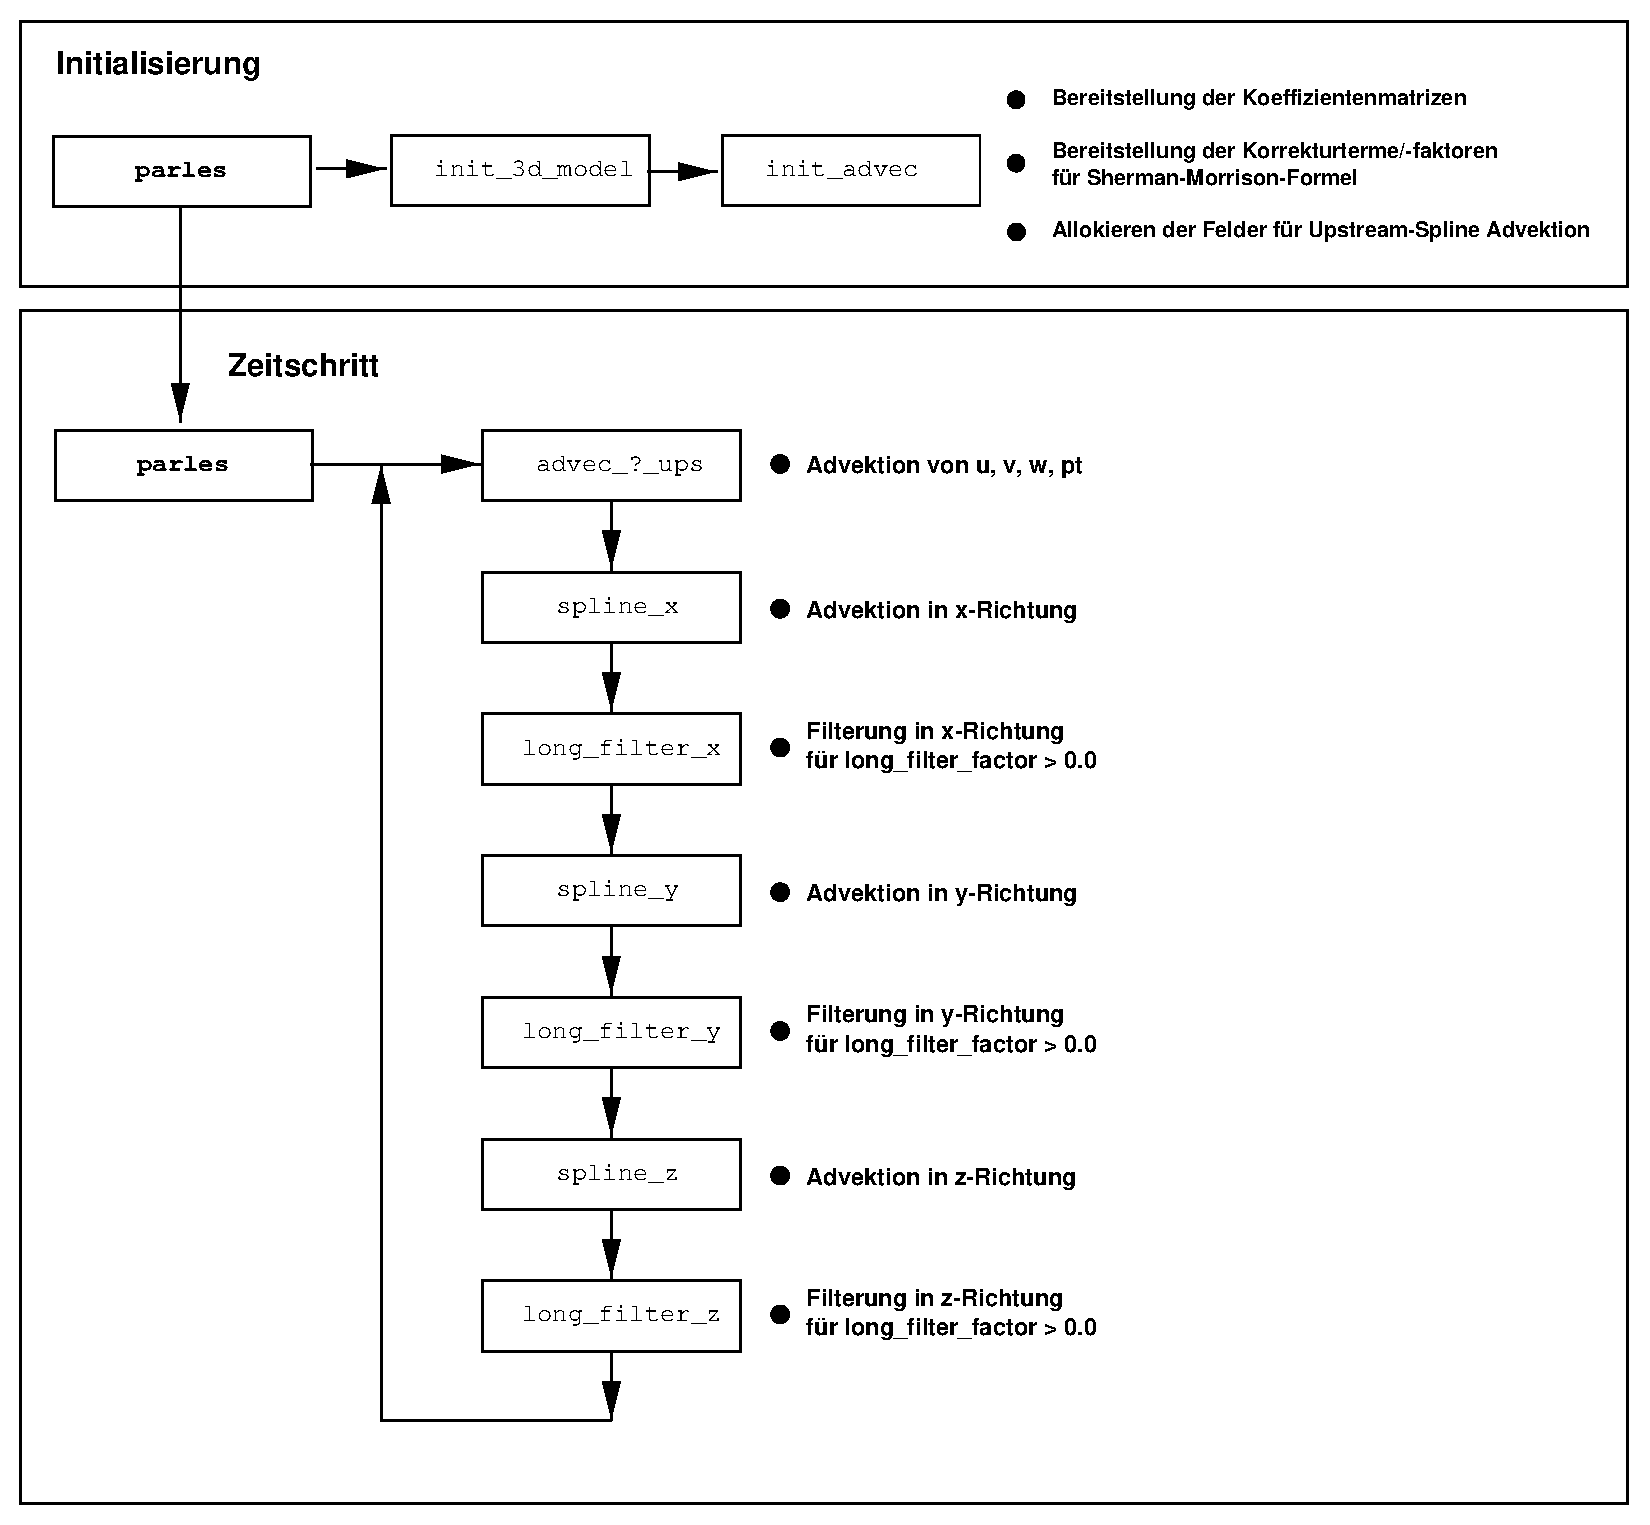
\includegraphics[width=\textwidth]{ablauf.eps}
\caption{Ablaufplan f"ur das Upstream-Spline Advektionsverfahren}
\label{ablauf:fig}
\end{figure}

\newpage
\bibliography{ups}

\end{document}

